%!TEX root = ../dissertation.tex
%\begin{savequote}[75mm]
%Nulla facilisi. In vel sem. Morbi id urna in diam dignissim feugiat. Proin molestie tortor eu velit. Aliquam erat %volutpat. Nullam ultrices, diam tempus vulputate egestas, eros pede varius leo.
%\qauthor{Quoteauthor Lastname}
%\end{savequote}

\chapter{Singular}
\label{chap:singular}

\emph{Singular} è la prima libreria di identificazione di ambienti virtualizzati che si basa nelle strutture del \emph{\gls{artg}} con valori ricavati direttamente dalla memoria centrale, basandosi su un metodo più  robusto ed efficace rispetto a quelli attualmente esistenti.
Gli studi effettuati e le conoscenze accumulate durante il periodo di stage hanno portato a velocizzare di molto la sua implementazione e realizzazione.

In questo capitolo verrà descritta la progettazione e l'implementazione di \emph{Singular}, la sua efficienza e la sua compatibilità, oltre a possibili contromisure.

\newpage

\section{Strumenti utilizzati}

\subsection*{Android Studio}

\emph{Android Studio} è l'\emph{\gls{ideg}}\glsfirstoccurspace primario di \emph{Google} per la realizzazione di applicazioni \emph{Android}. Integra molti strumenti utili per la realizzazione di pacchetti in modo professionale.
Di default integra principalmente:
\begin{itemize}
    \item compilazione flessibile con \emph{Gradle};
    \item editing di layout in modo grafico e veloce;
    \item \emph{app signer} e \emph{ProGuard};
    \item possibilità di creare \emph{APK} multipli;
    \item elementi di ispezione a runtime delle applicazioni;
    \item emulatore \emph{Android}.
\end{itemize}
Strumenti che consentono di sviluppare applicazioni \emph{Android} in modo veloce senza utilizzare componenti aggiuntivi.

\subsection*{Android SDK}

L'\emph{Android SDK} è il pacchetto di sviluppo per applicazioni \emph{Android} che viene implementato negli \emph{\gls{ideg}} come \emph{Android Studio}.
Ogni versione di \emph{Android} corrisponde a una specifica \emph{API} e per ognuna di essa c'è un corrispondente \emph{Android SDK Platform}, scaricabile direttamente dal gestore dei pacchetti di \emph{Android Studio}.



\subsection*{Android NDK}

L'\emph{Android NDK} o \emph{Android Native Development Kit} è il pacchetto di sviluppo per l'integrazione di codice a basso livello (C/C++) nelle applicazioni. \emph{Android Studio} permette di installarlo direttamente dal suo gestore dei pacchetti.

\subsection*{ADB}

L'\emph{Android Debug Bridge} è uno strumento utilizzato per comunicare con un dispositivo \emph{Android}, in modo da avviare debug di applicazioni tramite \emph{\gls{ideg}}, oppure semplicemente per lanciare dei comandi linux.
Viene installato insieme a \emph{Android Studio}.

\section{Analisi dei requisiti}

I requisiti individuati sono stati catalogati in Tab. \ref{tab:singular_req} secondo la seguente notazione:\\

\centerline{R[Tipo][Importanza][Codice]}\\

Dove:
\begin{itemize}
    \item \emph{Tipo} può assumere i seguenti valori:
    
    \emph{F}: funzionale, descrive le funzionalità della libreria\\
    \emph{V}: vincolo, descrive i vincoli imposti per la realizzazione della libreria\\
    \emph{P}: prestazionale, descrive i requisiti sulle prestazioni della libreria\\
    
    \item \emph{Importanza} può assumere i seguenti valori:
        
    \emph{0}: requisito obbligatorio\\
    \emph{1}: requisito desiderabile\\
    \emph{2}: requisito opzionale\\
    
    \item \emph{Codice} viene utilizzato per identificare univocamente il requisito tramite un numero progressivo.
    
\end{itemize}

\begin{table} [H]

\begin{tabular}{l|l}    \toprule
\emph{Codice}  & \emph{Descrizione} \\\midrule
\row RF01 & La libreria deve essere in grado di rilevare un ambiente virtualizzato. \\ 
\row RF02 & La libreria deve essere in grado di rilevare un ambiente reale. \\ 
\row RF03 & La libreria deve utilizzare codice nativo per leggere dalla memoria centrale. \\
\row RF04 & La libreria deve utilizzare le informazioni ricavate dalle strutture di ART. \\
\row RF15 & La libreria dovrebbe essere implementata all'interno di un'applicazione di prova. \\
\row RV06 & Fornire un insieme di test per dimostrare l'efficienza della libreria. \\
\row RV17 & Fornire un insieme di test utilizzando versioni di Android e dispositivi diversi. \\
\bottomrule \hline
\end{tabular}



\caption[Tabella dei requisiti di Singular]{Tabella dei requisiti di Singular}
\label{tab:singular_req}
\end{table}

\newpage

\section{Progettazione ed implementazione}

\emph{Singular} è composta da due parti principali: 
\begin{itemize}
    \item codice a basso livello C/C++
    \item codice Java
\end{itemize}

Il diagramma delle classi si può vedere in Fig. \ref{fig:singular_uml}.



\begin{figure} [H]
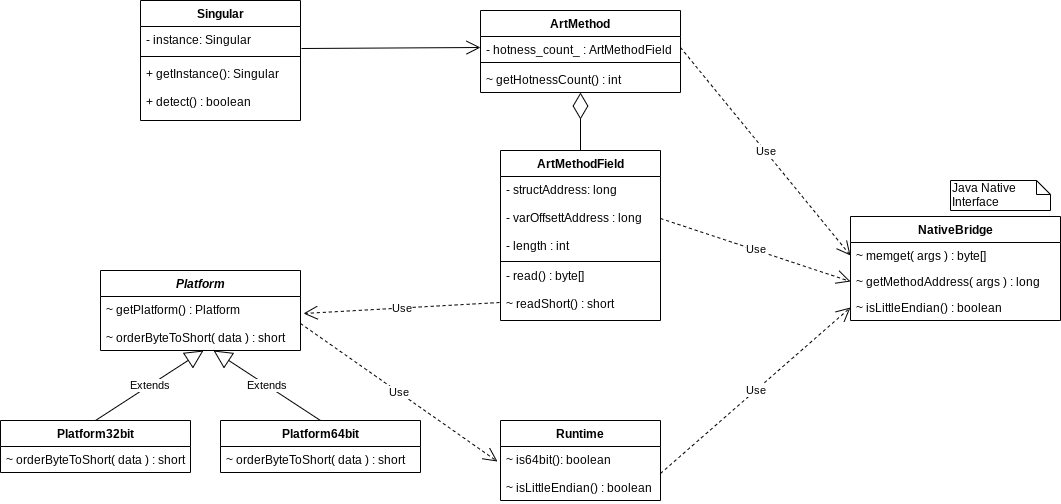
\includegraphics[width=1.2\textwidth]{figures/Singular}
\caption[Diagramma delle classi di Singular]{diagramma delle classi di Singular
\label{fig:singular_uml}}
\end{figure}

\subsection*{Codice nativo}

L'utilizzo del codice nativo C/C++ è necessario per poter leggere dalla memoria primaria l'indirizzo degli \emph{ArtMethod} e l'\emph{hotness\_count} a esso associato.
La classe \emph{Java} che implementa i metodi nativi attraverso la \emph{Java Native Interface} è \emph{NativeBridge}.

\begin{lstlisting}[language = Java , frame = trBL , firstnumber = 1 , escapeinside={(*@}{@*)}]
final class NativeBridge {
    static {
        System.loadLibrary("singularnative");
    }
    static native byte[] memget(long address, int size);
    static native long getMethodAddress(Method method);
    static native boolean isLittleEndian();
}
\end{lstlisting}

La classe è finale ed è raggiungibile solo dallo stesso package per evitare che sia accessibile dall'esterno.
I corrispondenti metodi dichiarati nella classe \emph{NativeBridge} sono disponibili all'interno della libreria \emph{SingularNative}, che viene caricata in riga 3. Le funzioni vengono implementate nel file \emph{singular\_native.cpp} in questo modo:
\begin{itemize}
    \item \emph{isLittleEndian()}
    \begin{lstlisting}[language = C , frame = trBL , firstnumber = 1 , escapeinside={(*@}{@*)}]
jboolean isLittleEndian(JNIEnv * env, jclass clazz) {
    unsigned int num = 0,*p = &num;
    *(unsigned char *)p = 0xff;
    if (num == 0xff)
        return JNI_TRUE;
    return JNI_FALSE;
}
\end{lstlisting}

Verifica se la CPU è \emph{little endian} provando a invertire i byte assegnando il valore \emph{0xff} a un puntatore a un intero.

    \item \emph{getMethodAddress(Method method)}
\begin{lstlisting}[language = C , frame = trBL , firstnumber = 1 , escapeinside={(*@}{@*)}]
jlong getMethodAddress(JNIEnv * env, jclass clazz, jobject method) {
    return (jlong) env->FromReflectedMethod(method);
}
\end{lstlisting}
Viene ritornato l'indirizzo dell'\emph{artMethod} tramite la funzione \emph{FromReflectedMethod} e convertendo il risultato in \emph{jlong}.

    \item \emph{memget(long address ,int size)}
\begin{lstlisting}[language = C , frame = trBL , firstnumber = 1 , escapeinside={(*@}{@*)}]
jbyteArray android_memget(JNIEnv *env, jclass _cls, jlong src, jint length) {
    jbyteArray dest = env->NewByteArray(length);
    if (dest == NULL)
        return NULL;
    unsigned char *destPnt = (unsigned char*)env->GetByteArrayElements(dest,0);
    unsigned char *srcPnt = (unsigned char*)src;
    for(int i = 0; i < length; ++i)
        destPnt[i] = srcPnt[i];
    env->ReleaseByteArrayElements(dest, (jbyte *)destPnt, 0);
    return dest;
}
\end{lstlisting}
Tramite la funzione \emph{NewByteArray} viene allocato un array di lunghezza \emph{length}. Poi viene creato il puntatore alla zona di memoria di destinazione attraverso la funzione \emph{GetByteArrayElements}, e viene copiato l'array sorgente nell'array destinazione.
Tramite la funzione \emph{ReleaseByteArrayElements} viene rilasciata la memoria, e infine ritornato l'array \emph{dest}.
\end{itemize}


\subsection*{Codice java}

Le operazione che esegue \emph{Singular} per leggere il valore dell'\emph{hotness\_count} si possono riassumere in:
\begin{enumerate}
    \item Recupero della classe \emph{ActivityThread} e del metodo \emph{currentActivityThread}:
\begin{lstlisting}[language = C , frame = trBL , firstnumber = 1 , escapeinside={(*@}{@*)}]
Class target = Class.forName("android.app.ActivityThread");
Method curActivityThread = target.getDeclaredMethod("currentActivityThread");
\end{lstlisting}
    \item Creazione di un nuovo oggetto \emph{ArtMethod}, contenente l'indirizzo dell'oggetto \emph{ActivityThread} e l'istanza di un oggetto \emph{ArtMethodField} contenente l'offset e la lunghezza del campo \emph{hotness\_count}:
\begin{lstlisting}[language = C , frame = trBL , firstnumber = 1 , escapeinside={(*@}{@*)}]
ArtMethod(Method associatedMethod) {
    long methodAddress = NativeBridge.getMethodAddress(associatedMethod);
    hotness_count_ = new ArtMethodField(methodAddress, HOTNESS_COUNT_OFFSET, HOTNESS_COUNT_LENGTH);
}
\end{lstlisting}    
    \item Lettura del campo \emph{hotness\_count} grazie al metodo \emph{read} della classe \emph{ArtMethodField}. Prima di eseguire questa operazione viene controllata l'architettura del sistema operativo, tramite la classe \emph{Platform}:
\begin{lstlisting}[language = C , frame = trBL , firstnumber = 1 , escapeinside={(*@}{@*)}]
private byte[] read() {
    return NativeBridge.memget(structAddress + varOffsetAddress,length);
}
\end{lstlisting}       

    \item Viene eseguito il codice nativo della funzione \emph{memget} e viene ritornato il valore legato all'\emph{hotness\_count}, sul quale controllare l'ambiente di esecuzione. Nel caso in cui l'ambiente di esecuzione fosse virtuale, viene segnalato sull'\emph{\gls{activityg}} dell'applicazione \emph{Singular} di supporto.
\end{enumerate}

\newpage


\section{Efficienza}

\emph{Singular} è stata testata su un ampia gamma di dispositivi diversi tra loro, con diverse applicazioni di virtualizzazione. I risultati sono visibili in Tab. \ref{tab:singular_device_tests}.
Nel caso l'applicazione di virtualizzazione non fosse compatibile con la versione di \emph{Android}, il campo della tabella è vuoto.


\begin{table} [H]

\makebox[1 \textwidth][c]{       %centering table
\resizebox{1.2 \textwidth}{!}{   %resize table


\begin{tabular}{l|lllllllllll}    \toprule
\emph{device}  & native & A1 & A2 & A3 & A4 & A5 & A6 & A7 & A8 & DroidPlugin & Màscara\\\midrule
\row Xiaomi mi10 - Android 10 arm64 & false & true & true & true &   & true & true &  &      \\ 
\row Xiaomi mi9 - Android 10 arm64 & false & true & true & true &   & true & true &  &      \\ 
\row Xiaomi mi9t - Android 9 arm64 & false & true & true & true &   & true & true &  & & true & true     \\ 
\row Xiaomi mi9t Pro - Android 10 arm64 & false & true & true & true &   & true & true &  &      \\ 
\row Oneplus 3 - Android 8.1 arm64 & false & true & true & true & true  & true & true & true & true & true & true    \\ 
\row Oneplus 6 - Android 10 arm64 & false & true & true & true &   & true & true &  &     \\ 
\row Oneplus 6t - Android 10 arm64 & false & true & true & true &   & true & true &  &      \\ 
\row Samsung Galaxy S8 - Android 9 arm64& false & true & true & true &   & true & true &  &  & true & true       \\ 
\row Samsung Galaxy A70 - Android 10 arm64 & false & true & true & true &   & true & true &  &     \\ 
\row Samsung Galaxy S4 i9505 - Android 8 (AOSP) armeabi-v7 & false & true & true & true & true  & true & true & true & true & true & true    \\ 
\row LG G4 - Android 8 arm64 & false & true & true & true & true  & true & true & true & true  & true & true    \\  \bottomrule \hline
\end{tabular}



}
}
\caption[Tabella dei test di Singular]{Tabella dei test di Singular \\ false se l’ambiente rilevato è nativo, true se l’ambiente rilevato è virtualizzato \\ A1 = com.lbe.parallel.intl \\ A2 = com.ludashi.dualspace \\ A3 = 
info.cloneapp.mochat.in.goast \\ A4 = 
com.parallel.space.lite \\ A5 =
com.exelliance.multiaccounts \\ A6 =
com.ludashi.superboost \\ A7 =
com.in.parallel.accounts \\ A8 =
com.polestar.domultiple}
\label{tab:singular_device_tests}
\end{table}



\emph{Singular} è stato progettato in modo da mitigare ogni possibilità di \emph{\gls{hookg}} cercando di utilizzare operatori logici al posto di metodi, i quali possono essere intercettati da framework come \emph{Whale}. 



\newpage
\section{Compatibilità}

\emph{Singular} è compatibile da \emph{Android Oreo 8.0} fino all'ultima versione rilasciata ufficialmente \emph{Android 10}. Come si può vedere in Fig. \ref{fig:androidOSdistribution} \emph{Singular} copre il 60.8\% dei dispositivi, percentuale sempre in aumento con il passare del tempo.

\begin{figure} [H]
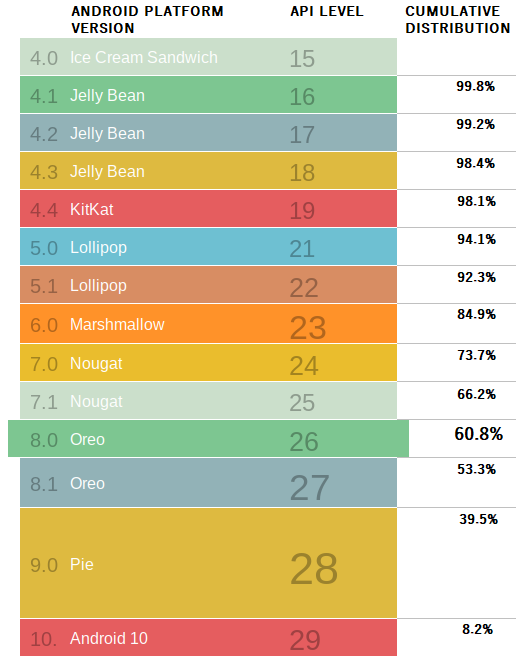
\includegraphics[width=0.8\textwidth]{figures/androidOSdistribution}
\caption[Distrubuzione di Android di Maggio 2020]{Distrubuzione di Android di Maggio 2020
\label{fig:androidOSdistribution}}
\end{figure}

Anche se la percentuale di compatibilità è ancora bassa, la verifica dell'\emph{hotness\_count} per il rilevamento di ambienti virtualizzati risulta essere una tecnica molto più robusta e affidabile rispetto a quelle implementate dalle attuali librerie di identificazione.

\section{Contromisure}

Una possibile contromisura potrebbe essere la riscrittura del valore del field \emph{hotness\_count} ai valori di \emph{Android} nativo. Attraverso il metodo \emph{mprotect} di linux è possibile rimuovere la protezione dalla corrispondente pagina di memoria. 
Le operazioni che dovrebbe eseguire un possibile malware per aggirare questa tecnica di identificazione di ambienti virtualizzati sono:
\begin{itemize}
    \item Implementazione di codice a basso livello per la scrittura in memoria e per la rimozione della protezione;
    \item Riscrittura di tutti gli \emph{hotness\_count} diversi in ambiente virtualizzato: implicherebbe un calo di performance non indifferente per l'applicazione vittima.
\end{itemize}

La fattibilità di una contromisura di questo tipo viene lasciata come test futuro.

\section{Verifica dei requisiti}

I requisiti richiesti iniziali sono stati tutti soddisfatti, come è possibile vedere in Tab. \ref{tab:sodd_requisiti}.


\begin{table} [H]

\begin{tabular}{l|l}    \toprule
\emph{Codice}  & \emph{Esito} \\\midrule
\row RF01 & Soddisfatto \\ 
\row RF02 & Soddisfatto \\ 
\row RF03 & Soddisfatto \\
\row RF04 & Soddisfatto \\
\row RF15 & Soddisfatto \\
\row RV06 & Soddisfatto \\
\row RV17 & Soddisfatto \\
\bottomrule \hline
\end{tabular}


\caption[Tabella del soddisfacimento dei requisiti di Singular]{Tabella del soddisfacimento dei requisiti di Singular}

\label{tab:sodd_requisiti}
\end{table}

